This chapter contains theoretical information about the paper's domain, deep learning, and the principal model used, autoencoders.
Of course, before starting looking in its domain, we should start with the basics, namely, machine learning.
\section{What is Machine Learning?}

Machine learning is one of many subfields of artificial intelligence, the science of getting the computer to learn from experience
without being explicitly programmed to do so, improving their ability to think, plan, decide, etc. \cite{whatIsML}.
\vspace{0.5cm}

Algorithms in this area are different in their approach, the type of data they input and output, and the type of problem they are learning to
solve, but, despite all differences, they are based on the same idea that there are some generic algorithms that can discover patterns,
without having to write code; instead, they build their own logic on the data fed to them.
\vspace{0.5cm}

One of the main types of machine learning algorithms that are vastly used is artificial neural networks or ANNs.
They are structured as weighted graphs, modelled after the human brain where each node represents a neuron and each
edge represents the synapses of the neural network. The weight of each edge determines how powerful the synapse is.
The neurons are distributed in groups named layers. Neurons can form synapses only with neurons from other layers.
\vspace{0.5cm}

As you can see in \emph{\ref{fig:ann_structure}} there are three types of layers in an artificial neural network:
\begin{itemize}[]
    \item{ Input layer
          \begin{adjustwidth}{1cm}{}
              This layer of a neural network is the very beginning of the ANN’s workflow, bringing the initial data into the system for
              further processing by subsequent layers of artificial neurons \cite{inputLayer}.
          \end{adjustwidth}
          }
    \item{ Hidden layer
          \begin{adjustwidth}{1cm}{}
              Any layer between the output and the input layer is considered to be a hidden layer.
              The number of neurons they contain and also their number can vary.
              Their role is to take in a set of weighted inputs and produce an output through an activation function \cite{hiddenlayer}.
          \end{adjustwidth}
          }
    \item{ Output layer
          \begin{adjustwidth}{1cm}{}
              This layer of a neural network is the last layer of neurons that produces given outputs for the program.
              They usually are made much like any other artificial neuron, but they may be observed in a different way,
              the output layer coalesces and concretely produces the end result \cite{outputLayer}.
          \end{adjustwidth}
          }
\end{itemize}
\begin{figure}[h]
    \centering
    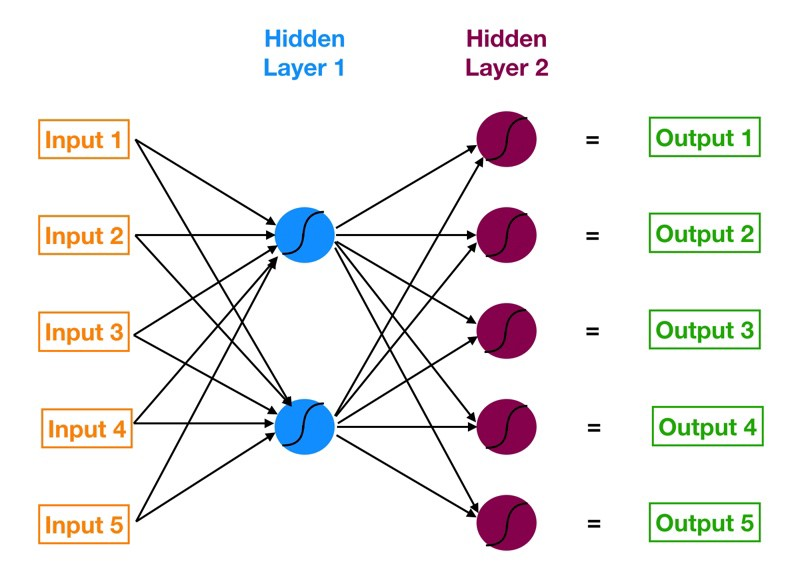
\includegraphics[width=1\textwidth]{ann_structure}
    \caption{\emph{Neural network with one hidden layer \cite{understandingANN}}}
    \label{fig:ann_structure}
\end{figure}


\section{What is Deep Learning?}

Deep learning is a subfield of machine learning that contains a collection of ANNs that are known for
their capability on learning unsupervised from data that is unstructured or unlabeled.
Also known as deep neural learning or deep neural network.
\vspace{0.5cm}

A second classification we can make on ANNs is based on the relationships between their nodes.
Then, neural networks can be recurrent or feedforward;
the first one does not have any loops in its graph and can be organized in layers.
A deep neural network is a feedforward ANN with many hidden layers
\vspace{5cm}

A visual representation of the aforementioned is the fig\emph{~\ref{fig:deep_vs_normal}} wherein we could see
the differences between a simple feedforward ANN with one hidden layer(left) and a deep neural network with three
hidden layers
\begin{figure}[h]
    \centering
    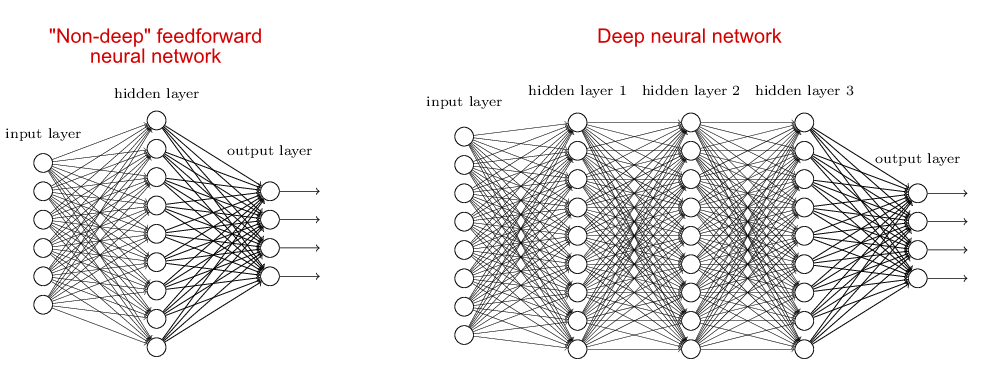
\includegraphics[width=1\textwidth]{deep_vs_normal_ann}
    \caption{\emph{Difference between a Non-deep ANN(left) and a deep ANN(right) \cite{deepLearningBook}}}
    \label{fig:deep_vs_normal}
\end{figure}

